

\section{Cards, Decks, and Hands: The Exponential Formula}
\begin{exercise}
    Give an explicit 1-1 correspondence between partitions of $n$ into distinct parts and partitions of $n$ into odd parts.
\end{exercise}
\begin{solution}
    The key idea is that any number can be uniquely expressed as a power of $2$ times an odd number (also used in Exercise~\ref{ex:2-25}).

    Now, suppose we have a partition of $n$ into odd parts:
    \[
        n = x_1 1+ x_3 3 + x_5 5 + \ldots
    \]
    and write each $x_i$ in binary (as a sum of distinct powers of two):
    \[
        n = (2^{b_{11}} + 2^{b_{12}} + \ldots)1 + (2^{b_{31}} + 2^{b_{32}} + \ldots)3 + \ldots
    \]
    Distributing over the brackets gives a partition of $n$ into distinct parts.

    This map is easily seen to be invertible, since from a partition into distinct parts one just writes every number as the product of a power of $2$ and an odd number and then writes the odd number that number of times.
\end{solution}

\begin{exercise}
    Fix integers $n,k$. Let $f(n,k)$ be the number of permutations of $n$ letters whose cycle lengths are all divisible by $k$. Find a simple, explicit egf for $\{f(n,k)\}_{n\geq 0}$. Find a simple, explicit formula for $f(n,k)$.
\end{exercise}
\begin{solution}
    Since only cycle lengths divisible by $k$ are allowed, only the decks $\mathcal{D}_{mk}$ will contain any cards (the cards are the usual ones for cycles of permutations). The $mk$th deck will contain $d_{mk} = (mk-1)!$ cards leading to the deck enumerator:
    \[
        \mathcal{D}(x) = \sum_{m=1}^\infty (mk-1)! \frac{x^{mk}}{(mk)!} = \frac{1}{k}\sum_{m=1}^\infty \frac{x^{mk}}{m} \estep{\eqref{eq:power_loggeom}} \frac{1}{k} \log\left(\frac{1}{1-x^k}\right)
    \]
    Let $\mathcal{H}_k(x) \stackrel{egf}{\longleftrightarrow} \{f(n,k)\}_{n\geq 0}$, where $f(n,k)$ is the number of permutations of $n$ letters whose cycles are all divisible by $k$. Then by the exponential formula:
    \[
        \mathcal{H}_k(x) = \exp\left\{ \frac{1}{k}\log\left(\frac{1}{1-x^k}\right)\right\} = \frac{1}{(1-x^k)^{\frac{1}{k}}}
    \]
    To find an explicit formula for $f(n,k)$, we need to find the coefficient of $\frac{x^n}{n!}$. Using \eqref{eq:binom_num} with $y=-x^k$ and $\alpha = -\frac{1}{k}$ yields:
    \begin{align*}
        f(n, k) = \coeff{\expcoeff}H_k(x) = \coeff{\frac{x^n}{n!}} \bsum[l] \binom{-\frac{1}{k}}{l} (-1)^l x^{kl}= \begin{cases}
            (-1)^{\frac{n}{k}} \displaystyle\binom{-\frac{1}{k}}{\frac{n}{k}}n!, & \textnormal{if $k\vert n$} \\
            0, & \textnormal{else}
        \end{cases}
    \end{align*}
    More precisely, when $n$ is a multiple of $k$, let $r = \frac{n}{k}$, then:
    \begin{align*}
        f(n,k) &= (-1)^r \binom{-\frac{1}{k}}{r}n! \\
        &= (-1)^r \frac{n!}{r!}\left(-\frac{1}{k}\right)\left(-\frac{1+k}{k}\right)\left(-\frac{1+2k}{k}\right)\cdots\left(-\frac{1+(r-1)k}{k}\right) \\
        &= \frac{n!}{r!k^r}(1+k)(1+2k)\cdots(1+(r-1)k)
    \end{align*}
\end{solution}

\begin{exercise}
    Find the egf for the partitions of the set $[n]$, all of whose classes have a prime number of elements.
\end{exercise}
\begin{solution}
    The usual cards for set partitions are used (cards with an arbitrary picture and a label set). Since only classes with a prime number of elements are allowed, $\mathcal{D}_k$ will contain one card if $k$ is prime and zero cards otherwise. Then, by the exponential formula, the egf for the number of partitions of the set $[n]$ is (we do not care about the number of classes):
    \[
        \exp\left\{\sum_{p} \frac{x^p}{p!} \right\}
    \]
    where $p$ loops over all primes.
\end{solution}

\begin{exercise}
    In a group $\Gamma$, the \emph{order} of an element $g$ is the least positive integer $\rho$ such that $g^\rho = 1_\Gamma$.
    \begin{enumerate}[label=(\alph*)]
        \item In the group of all permutations of $n$ letters, express the order of a permutation $\sigma$ in terms of the lengths of its cycles.
        \item Let $g(n,k)$ be the number of permutations of $n$ letters whose order is $k$. Express $g(n,k)$ in terms of the number $\tilde{g}(n,m)$ of $n$-permutations whose cycle lengths all divide $m$.
    \end{enumerate}
\end{exercise}
\begin{solution}
    \begin{enumerate}[label=(\alph*)]
        \item Since the cycles are disjoint, they commute and taking the $k$th power is equivalent to taking the $k$th power of each cycle. A cycle fixes all its elements if and only if its length is a divisor of $k$. The least integer such that all elements are fixed is the least common multiple of all the cycle lengths.
        \item We first express $\tilde{g}(n,m)$ in terms of $g(n,k)$:
        \[
            \tilde{g}(n,m) = \sum_{d\vert m} g(n,d)
        \]
        since every permutation whose order is $d$ has cycle lengths dividing $m$ which is a multiple of $d$. Applying M\"{o}bius inversion gives the desired result:
        \[
            g(n,k) = \sum_{d\vert k} \mu\left(\frac{n}{d}\right)\tilde{g}(n,d)
        \]
    \end{enumerate}
\end{solution}

\begin{exercise}
    \label{ex:3-5}
    Let $T_n$ be the number of involutions of $n$ letters.
    \begin{enumerate}[label=(\alph*)]
        \item Find a recurrence formula that is satisfied by these numbers.
        \item Compute $T_1,\ldots,T_6$.
        \item Give a combinatorial and constructive interpretation of the recurrence. That is, after having derived it from the generating function, re-derive it without the generating function.
    \end{enumerate}
\end{exercise}
\begin{solution}
    \begin{enumerate}[label=(\alph*)]
        \item The egf for the number of involutions of $n$ letters is:
        \[
            T(x) = \bsum[n] \frac{T_n}{n!}x^n = e^{x+\frac{1}{2}x^2}
        \]
        Taking the logarithm of both sides:
        \[
            \log\left( \bsum[n] \frac{T_n}{n!}x^n\right) = x+\frac{1}{2}x^2
        \]
        Differentiating both sides and multiplying by $T(x)x$:
        \[
            xT'(x) = T(x)(x+x^2)
        \]
        Equating coefficients of $\frac{x^n}{n!}$:
        \[
            nT_n = nT_{n-1} + n(n-1)T_{n-2}
        \]
        Dividing by $n$ and reading of the base cases from the egf:
        \[
            T_n = T_{n-1} + (n-1)T_{n-2},\quad (n\geq 2,\ T_0 = 1,\ T_1 = 1)
        \]
        \item From the recurrence relation, we find:
        \[
            T_1 = 1,\ T_2 = 2,\ T_3 = 4,\ T_4 = 10,\ T_5 = 26,\ T_6 = 76
        \]
        \item An involution is a composition of length $1$ and $2$ cycles. Now consider the involutions in which $n$ is in a length $1$ cycle (fixed point). There are $T_{n-1}$ of them. There are $(n-1)T_{n-2}$ involutions in which $n$ appears in a length $2$ cycle ($n-1$ possibilities for the other value and $T_{n-2}$ possibilities for all other $n-2$ values).
    \end{enumerate}
\end{solution}

\begin{exercise}
    Find, in simple form, the egf of the sequence of numbers of permutations of $n$ letters that have no cycles of lengths $\leq 3$. Your answer should not contain any infinite serires.
\end{exercise}
\begin{solution}
    Let the cards be the usual ones for cycles of permutations and the $n$th deck containing $d_n = (n-1)!$ cards for $n > 3$ and zero for $0<n\leq 3$. The deck enumerator is:
    \[
        \mathcal{D}(x) = \sum_{m=4}^\infty (m-1)! \frac{x^m}{m!} = \sum_{m=4}^\infty \frac{x^m}{m} \estep{\eqref{eq:power_loggeom}} -x -\frac{x^2}{2} - \frac{x^3}{3} + \log \frac{1}{1-x}
    \]
    By the exponential formula, the egf of the sequence of numbers of permutations of $n$ letters that have no cycles of length $\leq 3$ is then:
    \[
        e^{\mathcal{D}(x)} = \exp\left\{-x -\frac{x^2}{2} - \frac{x^3}{3} + \log \frac{1}{1-x}\right\} = \frac{\exp(-x-\frac{x^2}{2} - \frac{x^3}{3})}{1-x}
    \]
\end{solution}

\begin{exercise}
    \label{ex:3-7}
    Find the generating function for labeled graphs with all vertices of degrees $1$ or $2$ and an odd number of connected components. Find a recurrence formula for these numbers, calculate the first few, and draw the graphs involved.
\end{exercise}
\begin{solution}
    Every card has a connected graph such that all vertices have degree $1$ or $2$. This is either a cycle or a path. For $n\leq 2$, there are no cycles and for $n\geq 3$, there are $\frac{(n-1)!}{2}$ cycles (corresponding to the number of undirected circular arrangements).

    For $n\geq 2$, there are $\frac{n!}{2}$ paths (the number of undirected linear arrangements). We therefore have:
    \[
        d_n = \begin{cases}
            0 &  n < 2 \\
            1 & n = 2 \\
            \frac{n!}{2} + \frac{(n-1)!}{2} & n \geq 3
        \end{cases}
    \]
    The deck enumerator is therefore:
    \[
        \mathcal{D}(x) = \frac{x^2}{2} + \frac{1}{2}\sum_{m=3}^\infty m!\frac{x^m}{m!} + \frac{1}{2} \sum_{m=3}^\infty (m-1)!\frac{x^m}{m!} = \frac{x^2}{2} + \frac{1}{2}\sum_{m=3}^\infty x^m + \frac{1}{2} \sum_{m=3}^\infty\frac{x^m}{m}
    \]
    Adding and subtracting the remaining terms from the summations until the geometric series \eqref{eq:power_geom} or the power series of $\log\frac{1}{1-x}$ \eqref{eq:power_loggeom} are found:
    \begin{align*}
        \mathcal{D}(x) &= \frac{x^2}{2} + \left(-\frac{1}{2} - \frac{1}{2}x - \frac{1}{2}x^2 + \frac{1}{2}\frac{1}{1-x}\right) + \left(-\frac{1}{2}x - \frac{1}{4}x^2 + \frac{1}{2}\log\frac{1}{1-x}\right) \\
        &= -\frac{1}{2} - x - \frac{1}{4}x^2 + \frac{1}{2}\frac{1}{1-x} + \frac{1}{2}\log\frac{1}{1-x}
    \end{align*}
    Since we want to count only graphs with an odd number of connected components, we use the exponential formula with number of cards restricted. Let $e_T(x) = \sum_{n\in T} \frac{x^n}{n!}$ where $T$ is the set of odd positive integers, then:
    \[
        e_T(x) = \bsum[k] \frac{x^{2k+1}}{(2k+1)!} \estep{\eqref{eq:power_sinh}} \sinh(x)
    \]
    Denote the generating function for labeled graphs with all vertices of degrees $1$ or $2$ and an odd number of connected components as $\mathcal{G}(x)$, then:
    \[
        \mathcal{G}(x) = \sinh(\mathcal{D}(x)) = \sinh\left(-\frac{1}{2} - x - \frac{1}{4}x^2 + \frac{1}{2}\frac{1}{1-x} + \frac{1}{2}\log\frac{1}{1-x}\right)
    \]
    We derive a general recurrence relation for hands with an odd number of cards where $\mathcal{H}(x)$ is the hands enumerator and $\mathcal{D}(x)$ is the deck enumerator. From the exponential formula:
    \[
        \mathcal{H}(x) = \sinh(\mathcal{D}(x))
    \]
    Applying logarithm to both sides and differentiating, and then multiplying both sides by $x\mathcal{H}(x)$ yields:
    \[
        \Longleftrightarrow \frac{\mathcal{H}'(x)}{\mathcal{H}(x)} = \coth(\mathcal{D}(x))\mathcal{D}'(x) \Longleftrightarrow x\mathcal{H}'(x) = x\cosh(\mathcal{D}(x))\mathcal{D}'(x)
    \]
    Define $\mathcal{K}(x) = \cosh(\mathcal{D}(x))$ and equate coefficients of $\frac{x^n}{n!}$:
    \[
        nh_n = \bsum[l]\binom{n}{l}k_{n-l}ld_{l}
    \]
    We now derive a formula for $k_n$:
    \[
        \bsum[m] k_m \frac{x^m}{m!} = \cosh(\mathcal{D}(x))
    \]
    Differentiating both sides and multiplying by $x$ gives:
    \[
        \bsum[m] k_m m \frac{x^m}{m!} = x\sinh(\mathcal{D}(x))\mathcal{D}'(x) = x\mathcal{H}(x)\mathcal{D}'(x)
    \]
    Equating coefficients of $\frac{x^n}{n!}$ gives:
    \[
        nk_n = \bsum[m] \binom{n}{m} h_{n-m}md_m 
    \]
    with $k_0 = 1$ due to the expansion of $\cosh$ and the fact that $\mathcal{D}(x)$ has a zero constant term.

    Combining this formula with the previous formula gives a recurrence relation for the unknowns $h_n$ (only considering the range of nonzero values for the summand):
    \begin{align*}
        nh_n &= nd_n + \sum_{l=1}^{n-1} \sum_{m=1}^{n-l} \binom{n}{l}ld_l \frac{1}{n-l}\binom{n-l}{m}h_{n-l-m}md_m
    \end{align*}
    with $h_0 = 0$ due to the expansion of $\sinh$ and the fact that $\mathcal{D}(x)$ has a zero constant term.

    Applying the recurrence formula for $\mathcal{G}(x)$ gives:
    \[
        g_0 = 0,\ g_1 = 0,\ g_2 = 1,\ g_3 = 4,\ g_4 = 15,\ g_5 = 72,\ g_6 = 435,\ g_7 = 3300
    \]
    \[
        g_8 = 30310,\ g_9 = 322336,\ g_{10} = 3845520,\ g_{11} = 50459040
    \]
    Figure \ref{fig:3:7} shows some of the involved graphs which are counted.
    \begin{figure}[hbpt]
    \centering
    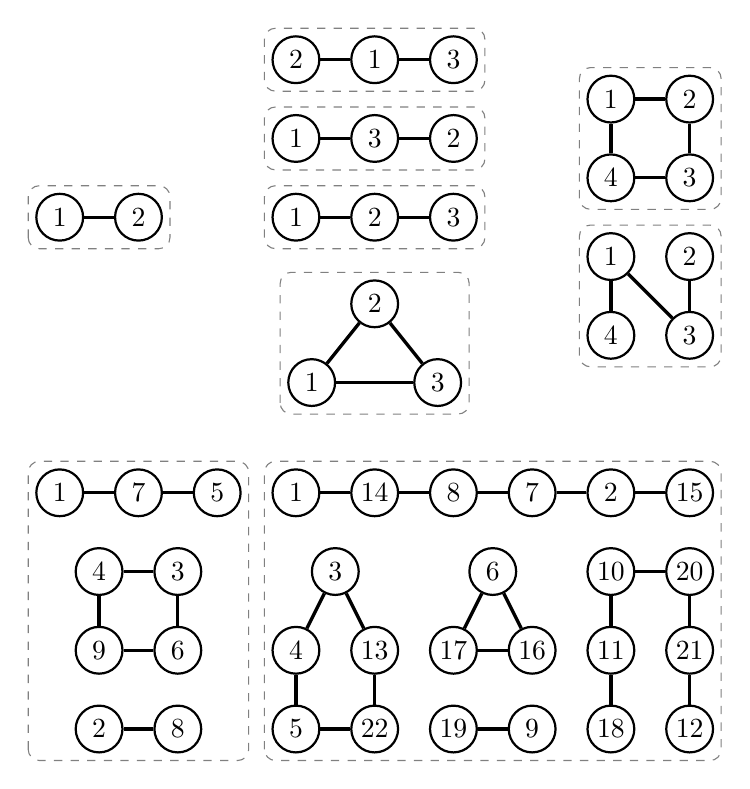
\begin{tikzpicture}
        \begin{scope}[every node/.style={circle,thick,draw,inner sep=0pt, text width=5.5mm, align=center}]
            \node (A1) at (-10,0) {1};
            \node (A2) at (-9,0) {2};

            \node (B1) at (-7, 0) {1};
            \node (B2) at (-6, 0) {2};
            \node (B3) at (-5, 0) {3};

            \node (C1) at (-7, 1) {1};
            \node (C2) at (-6, 1) {3};
            \node (C3) at (-5, 1) {2};

            \node (D1) at (-7, 2) {2};
            \node (D2) at (-6, 2) {1};
            \node (D3) at (-5, 2) {3};

            \node (E1) at (-6.8, -2.1) {1};
            \node (E2) at (-6, -1.1) {2};
            \node (E3) at (-5.2, -2.1) {3};

            \begin{scope}[shift={(0, -0.5)}]
            \node (F1) at (-3, 0) {1};
            \node (F2) at (-2, 0) {2};
            \node (F3) at (-2, -1) {3};
            \node (F4) at (-3, -1) {4};

            \node (G1) at (-3, 2) {1};
            \node (G2) at (-2, 2) {2};
            \node (G3) at (-2, 1) {3};
            \node (G4) at (-3, 1) {4};
            \end{scope}

            \begin{scope}[shift={(0,1.5)}]
            \node (H1) at (-10, -5) {1};
            \node (H7) at (-9, -5) {7};
            \node (H5) at (-8, -5) {5};
            \begin{scope}[shift={(0.5,0)}]
            \node (H4) at (-10, -6) {4};
            \node (H3) at (-9, -6) {3};
            \node (H6) at (-9, -7) {6};
            \node (H9) at (-10, -7) {9};
            \node (H2) at (-10, -8) {2};
            \node (H8) at (-9, -8) {8};
            \end{scope}
            \end{scope}

            \node (I1) at (-7, -3.5) {1};
            \node (I14) at (-6, -3.5) {14};
            \node (I8) at (-5, -3.5) {8};
            \node (I7) at (-4, -3.5) {7};
            \node (I2) at (-3, -3.5) {2};
            \node (I15) at (-2, -3.5) {15};
            
            \node (I3) at (-6.5, -4.5) {3};
            \node (I5) at (-7, -6.5) {5};
            \node (I4) at (-7, -5.5) {4};
            \node (I13) at (-6, -5.5) {13};
            \node (I22) at (-6, -6.5) {22};

            \node (I6) at (-4.5, -4.5) {6};
            \node (I17) at (-5, -5.5) {17};
            \node (I16) at (-4, -5.5) {16};

            \node (I19) at (-5, -6.5) {19};
            \node (I9) at (-4, -6.5) {9};

            \node (I10) at (-3, -4.5) {10};
            \node (I11) at (-3, -5.5) {11};
            \node (I18) at (-3, -6.5) {18};
            \node (I20) at (-2, -4.5) {20};
            \node (I21) at (-2, -5.5) {21};
            \node (I12) at (-2, -6.5) {12};
        \end{scope}

        \draw[rounded corners, draw=gray, dashed] (-10.4, -0.4) rectangle ++(1.8, 0.8);
        \draw[rounded corners, draw=gray, dashed] (-7.4, -0.4) rectangle ++(2.8, 0.8);
        \draw[rounded corners, draw=gray, dashed] (-7.4, 0.6) rectangle ++(2.8, 0.8);
        \draw[rounded corners, draw=gray, dashed] (-7.4, 1.6) rectangle ++(2.8, 0.8);
        \draw[rounded corners, draw=gray, dashed] (-7.2, -2.5) rectangle ++(2.4, 1.8);

        \draw[rounded corners, draw=gray, dashed] (-3.4, -1.9) rectangle ++(1.8, 1.8);
        \draw[rounded corners, draw=gray, dashed] (-3.4, 0.1) rectangle ++(1.8, 1.8);

        \draw[rounded corners, draw=gray, dashed] (-10.4, -6.9) rectangle ++(2.8, 3.8);

        \draw[rounded corners, draw=gray, dashed] (-7.4, -6.9) rectangle ++(5.8, 3.8);

        \begin{scope}[every edge/.style={draw=black, very thick}]
            \path [-] (A1) edge (A2);
            \path [-] (B1) edge (B2);
            \path [-] (C1) edge (C2);
            \path [-] (D1) edge (D2);
            \path [-] (E1) edge (E2);
            \path [-] (B2) edge (B3);
            \path [-] (C2) edge (C3);
            \path [-] (D2) edge (D3);
            \path [-] (E2) edge (E3);
            \path [-] (E1) edge (E3);
            \path [-] (F1) edge (F3);
            \path [-] (F1) edge (F4);
            \path [-] (F3) edge (F2);
            \path [-] (G1) edge (G2);
            \path [-] (G3) edge (G2);
            \path [-] (G3) edge (G4);
            \path [-] (G1) edge (G4);
            \path [-] (H1) edge (H7);
            \path [-] (H7) edge (H5);
            \path [-] (H4) edge (H3);
            \path [-] (H9) edge (H6);
            \path [-] (H9) edge (H4);
            \path [-] (H3) edge (H6);
            \path [-] (H2) edge (H8);

            \path [-] (I1) edge (I14);
            \path [-] (I14) edge (I8);
            \path [-] (I8) edge (I7);
            \path [-] (I7) edge (I2);
            \path [-] (I2) edge (I15);
            \path [-] (I3) edge (I4);
            \path [-] (I3) edge (I13);
            \path [-] (I4) edge (I5);
            \path [-] (I5) edge (I22);
            \path [-] (I22) edge (I13);
            \path [-] (I6) edge (I17);
            \path [-] (I6) edge (I16);
            \path [-] (I17) edge (I16);
            \path [-] (I19) edge (I9);
            \path [-] (I10) edge (I20);
            \path [-] (I10) edge (I11);
            \path [-] (I11) edge (I18);
            \path [-] (I20) edge (I21);
            \path [-] (I21) edge (I12);
        \end{scope}
    \end{tikzpicture}
    \caption{Some of the involved graphs in Exercise \ref{ex:3-7}}
    \label{fig:3:7}
    \end{figure}
\end{solution}

\begin{exercise}
    \label{ex:3-8}
    From 
    \[
        \sum_k \stirlingFst{n}{k} y^k = \coeff{\frac{x^n}{n!}}(1-x)^{-y} = n! \binom{y+n-1}{n} = y(y+1)\cdots (y+n-1)
    \] find a three term recurrence relation that is satisfied by the Stirling numbers of the first kind. Give a direct combinatorial proof of this recurrence relation. That is, reprove it, without using any generating functions.
\end{exercise}
\begin{solution}
    Note that:
    \[
        y(y+1)\cdots (y+n-1) = y(y+1)\cdots(y+n-2)y + y(y+1)\cdots (y+n-2)(n-1)  
    \]
    by the distributive property (split $y+n-1$ as $y + (n-1)$). Taking the coefficient corresponding to $y^k$ of each side gives:
    \[
        \stirlingFst{n}{k} = \coeff{y^k} \left(\bsum[k] \stirlingFst{n-1}{k}y^{k+1} + \stirlingFst{n-1}{k}y^k(n-1)\right) = \stirlingFst{n-1}{k-1} + (n-1)\stirlingFst{n-1}{k}
    \]
    For a combinatorial proof, we consider the cycle in which $n$ occurs. If it is a singleton cycle, there are $\stirlingFst{n-1}{k-1}$ configurations of the other elements. Otherwise, it occurs in one of the $k$ existing cycles. There are $(n-1)$ possibilities for the location (immediately following any of the other values) and $\stirlingFst{n-1}{k}$ configurations.
\end{solution}

\begin{exercise}
    Find the egf of the numbers $\{g(n)\}_0^\infty$ of permutations of $n$ letters that have both of the following properties: (a) they have an odd number of cycles and (b) the lengths of all of their cycles are even. Find a simple, explicit formula for these numbers.
\end{exercise}
\begin{solution}
    Take as cards the usual ones corresponding to cycles of permutations. The only decks with cards are the even-indexed ones with $d_{2n} = (2n-1)!$ such that the deck enumerator is
    \[
        \mathcal{D}(x) = \sum_{n = 1}^{\infty} (2n-1)!\frac{x^{2n}}{(2n)!} = \sum_{n = 1}^\infty \frac{x^{2n}}{2n} = \frac{1}{2} \sum_{n=1}^\infty \frac{(x^2)^n}{n} \estep{\eqref{eq:power_loggeom}} \frac{1}{2} \log \frac{1}{1-x^2}
    \]
    The hands enumerator follows from the exponential formula with number of cards restricted to an odd number using:
    \[
        e_T(x) = \bsum[t] \frac{x^{2t+1}}{(2t+1)!} \estep{\eqref{eq:power_sinh}} \sinh(x)
    \]
    The egf for the permutations that satisfies both properties is therefore:
    \begin{align*}
        \bsum g(n) \frac{x^n}{n!} &= \sinh\left(\log\frac{1}{\sqrt{1-x^2}}\right) = \frac{\frac{1}{\sqrt{1-x^2}} - \sqrt{1-x^2}}{2} = \frac{x^2}{2\sqrt{1-x^2}}
    \end{align*}
    To find a simple, explicit formula, we apply the binomial expansion:
    \begin{align*}
        g(n) &= \coeff{\frac{x^n}{n!}} \frac{x^2}{2\sqrt{1-x^2}} \\
        \estepalign{\eqref{eq:binom_num}} \coeff{\frac{x^n}{n!}} \frac{x^2}{2} \bsum[k] \binom{-\frac{1}{2}}{k}(-x^2)^k \\
        &= \coeff{\frac{x^n}{n!}}\frac{1}{2} \bsum[k] (-1)^k \binom{-\frac{1}{2}}{k} x^{2k + 2} \\
        &= \begin{cases}
            0 & \textnormal{if $n$ is odd} \\
            \frac{(-1)^{\frac{n}{2} - 1} n!}{2} \displaystyle\binom{-\frac{1}{2}}{\frac{n}{2} - 1} & \textnormal{if $n$ is even}
        \end{cases}
    \end{align*}
    Such that we can work with integer arithmetic on a computer, we rewrite the binomial such that the numerator is an integer. Let $n$ be even and $r = \frac{n}{2}$, then:
    \[
       g(n) = \frac{(-1)^{r - 1} n!}{2} \displaystyle\binom{-\frac{1}{2}}{r - 1}
    \]
    Using the generalized definition of the binomial:
    \[
        g(n) = \frac{(-1)^{r - 1} n!}{2(r-1)!}\left(-\frac{1}{2}\right)\left(-\frac{1}{2} - 1\right) \cdots \left(-\frac{1}{2}-r+2\right)
    \] 
    Factoring out $\frac{-1}{2}$ from each term:
    \[
        g(n) = \frac{(-1)^{r-1}n!}{2(r-1)!}\frac{(-1)^{r-1}}{2^{r-1}}(1)(1+2)\cdots(1+2r-4) = \frac{n!}{2^r(r-1)!}(1)(3)\cdots (n-3) 
    \]
    Multiplying and dividing by the even terms such that a factorial and subsequently a binomial coefficient can be recognized (also recall that $2r=n$):
    \begin{align*}
        g(n) &= \frac{n!}{2^r(r-1)!}(1)(3)\cdots(n-3) \frac{(2)(4)\cdots(n-2)}{(2)(4)\cdots(n-2)} \\
        &=  \frac{n!}{2^r(r-1)!} (n-2)! \frac{1}{2^{r-1}(1)(2)\cdots (r-1)} \\
       &= \frac{n!}{2^{n-1}} \binom{n-2}{r-1}
    \end{align*} 
\end{solution}

\begin{exercise}
    Find an explicit formula for $\stirlingSnd{n}{k}$, the Stirling numbers of the second kind by expanding the $k$th power that appears in 
    \[
        \stirlingSnd{n}{k} = \coeff{\frac{x^n}{n!}}\left\{\frac{(e^x-1)^k}{k!}\right\}
    \]
    by the binomial theorem. Your formula should be in the form of a single finite sum.
\end{exercise}
\begin{solution}
    Applying the binomial theorem gives:
    \begin{align*}
        \stirlingSnd{n}{k} &= \coeff{\frac{x^n}{n!}}\left\{\frac{(e^x-1)^k}{k!}\right\} \\
        \estepalign{\eqref{eq:binom_num}} \coeff{\frac{x^n}{n!}} \frac{1}{k!} \bsum[m] \binom{k}{m} e^{xm} (-1)^{k-m} \\
        &=  \bsum[m]\binom{k}{m} \frac{(-1)^{k-m}}{k!} \coeff{\frac{x^n}{n!}}e^{xm} \\
        &= \bsum[m] \binom{k}{m} \frac{(-1)^{k-m}m^n}{k!}
    \end{align*}
    Writing it as a finite sum by discarding the values for which the summand becomes $0$:
    \[
        \stirlingSnd{n}{k} = \sum_{m=0}^{k} \frac{(-1)^{k-m}m^n}{m!(k-m)!}
    \]
\end{solution}

\begin{exercise}
    Let $S$, $T$ be fixed sets of positive integers. Let $f(n;S,T)$ be the number of partitions of $[n]$ whose class sizes all lie in $S$ and whose number of classes lie in $T$. Show that $\{f(n;S,T)\}_{n\geq0}$ has the egf $e_T(e_S(x))$, where $e_S(x) = \sum_{s\in S} \frac{x^s}{s!}$.
\end{exercise}
\begin{solution}
    The cards are the usual ones for set partitions. Since every deck corresponding to a permittable class size has one card, the deck enumerator is:
    \[
        \mathcal{D}(x) = \sum_{s\in S} 1 \cdot \frac{x^s}{s!} = e_S(x)
    \]
    The exponential formula with restricted number of cards (number of classes), then immediately gives the asked answer:
    \[
        \bsum f(n;S,T) \frac{x^n}{n!} = e_T(e_S(x))
    \]
\end{solution}

\begin{exercise}
    Fix $k>0$. Let $f(n,k)$ be the number of permutations of $n$ letters whose longest cycle has length $k$. Find the egf of $\{f(n,k)\}_{n\geq0}$, for $k$ fixed.
\end{exercise}
\begin{solution}
    Let $g(n,k)$ be the number of permutations of $n$ letters whose cycles have lengths $\leq k$. Then the answer is given by $g(n,k) - g(n,k-1)$.

    As cards, we use the usual ones corresponding to cycles of permutations. Only cycle lengths $\leq k$ are allowed, so the deck enumerator is:
    \[
        \mathcal{D}(x) = \sum_{m=1}^k (m-1)! \frac{x^m}{m!} = \sum_{m=1}^k \frac{x^m}{m}
    \]
    Then, by the exponential formula:
    \[
        \bsum g(n,k) \frac{x^n}{n!} = \exp\left(\sum_{m=1}^k \frac{x^m}{m}\right)
    \]
    and:
    \begin{align*}
        \bsum f(n,k) \frac{x^n}{n!} &= \exp\left(\sum_{m=1}^k \frac{x^m}{m}\right) - \exp\left(\sum_{m=1}^{k-1} \frac{x^m}{m}\right) \\
        &= \exp\left(\sum_{m=1}^{k-1} \frac{x^m}{m}\right) \left(\exp\left(\frac{x^k}{k}\right) - 1\right)
    \end{align*}
\end{solution}

\begin{exercise}
    If $T(x)$ and $\mathcal{G}(x)$ denote, respectively, the egf's of involutions:
    \[
        T(x) = \sum_{n\geq 0}t_n\frac{x^n}{n!} = e^{x+\frac{1}{2}x^2}
    \]
    and of 2-regular graphs:
    \[
        \mathcal{G}(x) = \sum_{n\geq0}g(n) \frac{x^n}{n!}  = \frac{e^{-\frac{1}{2}x-\frac{1}{4}x^2}}{\sqrt{1-x}}
    \]
    then observe that:
    \[
        T(x)\mathcal{G}(x)^2 = \frac{1}{1-x}
    \]
    \begin{enumerate}[label=(\alph*)]
        \item Write out the identity between the sequences $\{g(n)\}$ and $\{t(n)\}$ that is implied by the above generating function relation.
        \item Show that for each fixed $n\geq1$ there are exactly the same numbers of
        \begin{enumerate}[label=(\roman*)]
            \item permutations of $n$ letters and of
            \item triples $(\tau,G_1,G_2)$, where $\tau$ is an involution of a set $R$, $G_1$ is a $2$-regular graph on a vertex set $S$, $G_2$ is a $2$-regular graph on a vertex set $T$, and $R$, $S$, $T$ partition $[n]$.
        \end{enumerate}
        \item Find, explicitly, a 1-1 correspondence such as is described in part (b) above.
    \end{enumerate}
\end{exercise}
\begin{solution}
    \begin{enumerate}[label=(\alph*)]
        \item Equating coefficients of $\frac{x^n}{n!}$ on both sides gives:
        \[
            \coeff{\frac{x^n}{n!}}\sum_{r,s,t \geq 0} t_r \frac{x^r}{r!} g_s \frac{x^s}{s!} g_t\frac{x^t}{t!} = \coeff{\frac{x^n}{n!}} \sum_{k\geq 0} x^k \Longleftrightarrow \sum_{r+s+t=n} \frac{n!}{r!s!t!}t_rg_sg_t = n!
        \]
        \item The multinomial coefficient gives the number of ways of partitioning $[n]$ into three parts, with $r$ numbers in the first part, $s$ in the second part and $t$ in the third part. $t_r$ counts the number of involutions which gets relabeled by the numbers in that class $R$. Similarly, $g_s$ and $g_t$ count the number of $2$-regular graphs relabeled using their respective classes.
        
        Adding these over all possible class sizes which sum to $n$ gives the left side. The number of permutations is on the right side.
        \item We give a construction from a triplet $(\tau, G_1, G_2)$ to a permutation $\sigma$. All involutions of $\tau$ will be mapped to the same cycles in $\sigma$. This will be one-to-one since $2$-regular graphs with cycle lengths of $2$ or less are impossible. Therefore from a permutation $\sigma$, its fixed points and length $2$-cycles in its cycle decomposition are in unique correspondence with $\tau$.
        
        Now for each cycle in $G_1$, we start from its smallest element (it doesn't matter from where a cycle in a permutation starts due to cyclic invariance) and map the cycle in the graph to a cycle in $\sigma$. There are $2$ ways to traverse the cycle in the graph. Let $G_1$ always go in the direction of the smallest element and $G_2$ in the direction of the largest element. Note that this construction is uniquely invertible since for every cycle in $\sigma$, we check the second element and the last element for which one is the largest which fixes the choice of $G_1$ and $G_2$ and the cycle in the corresponding graph.
    \end{enumerate}
\end{solution}

\begin{exercise}
    Let $\mathcal{F}$ be an exponential family with associated polynomials $\{\phi_n(x)\}$ of binomial type and with deck enumerator $\mathcal{D}(x)$.
    \begin{enumerate}[label=(\alph*)]
        \item If $D_y$ denotes the differential operator $\partial/\partial y$, then show that
        \[
            \mathcal{D}^{(-1)}(D_y)\phi_n(y) = n\phi_{n-1}(y) \quad (n\geq 0)
        \]
        by directly applying the operator to the egf of the polynomial sequence (here $\mathcal{D}^{-1}$ denotes the inverse function in the sense of functional composition).
        \item In the case of the exponential family of permutations by cycles, find the associated polynomials of binomial type, and verify the identity proved in part (a) by direct computation with those polynomials.
    \end{enumerate}
\end{exercise}
\begin{solution}
    \begin{enumerate}[label=(\alph*)]
        \item The polynomials of binomial type satisfy the generating relation:
        \[
            e^{y\mathcal{D}(x)} = \bsum \phi_n(y)\frac{x^n}{n!}
        \]
        Applying $D_y$ to the left side adds a factor of $\mathcal{D}(x)$ to the front. Applying a function $f(D_y)$ is therefore equivalent to multiplying by $f(\mathcal{D}(x))$. Choosing $f$ to be $\mathcal{D}^{-1}$ therefore multiplies the left side by $\mathcal{D}^{(-1)}(\mathcal{D}(x)) = x$. We now find:
        \[
            \mathcal{D}^{(-1)}(D_y) \bsum \phi_n(y) \frac{x^n}{n!} = x\bsum \phi_n(y) \frac{x^n}{n!} = \sum_{n=1}^\infty \phi_{n-1}(y)\frac{x^n}{(n-1)!}
        \]
        Equating coefficients of $\frac{x^n}{n!}$ gives the desired relation.
        \item The deck enumerator of permutations by cycles is:
        \[
            \mathcal{D}(x) = \log\frac{1}{1-x} \quad \textnormal{with inverse} \quad  \mathcal{D}^{(-1)}(x) = 1-e^{-x}
        \]
        The associated polynomials of binomial type are found from:
        \[
            e^{y\mathcal{D}(x)} = \frac{1}{(1-x)^y} \estep{\eqref{eq:binom_num}} \bsum \binom{-y}{n}(-x)^n = \bsum y(y+1)\cdots (y+n-1) \frac{x^n}{n!}
        \]
        \[
            \implies \phi_n(y) = y(y+1)\cdots (y+n-1)
        \]
        Now, the left-hand side of the relation is:
        \[
            \mathcal{D}^{(-1)}(D_y)\phi_n(y) = \phi_n(y) - e^{-D_y}\phi_n(y) = \phi_n(y) - \bsum[k] \frac{(-1)^k D_y^k}{k!}\phi_n(y) 
        \]
        We can write this last term in a more suggestive form
        \[
            \mathcal{D}^{(-1)}(D_y)\phi_n(y) = \phi_n(y) - \bsum[k] \frac{((y-1) - y)^k}{k!} D_y^k\phi_n(y)
        \]
        The sum is $\phi_n(y-1)$ from Taylor's theorem. We therefore have:
        \[
            \mathcal{D}^{(-1)}(D_y)\phi_n(y) = \phi_n(y) - \phi_n(y-1)
        \]
        Plugging in the polynomials:
        \begin{align*}
            \mathcal{D}^{(-1)}(D_y)\phi_n(y) &= y(y+1)\cdots (y+n-1) - (y-1)y\cdots (y+n-2) \\
            &= y(y+1)\cdots(y+n-2)\big\{y+n-1 - (y-1)\big\} \\
            &= y(y+1)\cdots (y+n-2)n \\
            &= n\phi_{n-1}(y)
        \end{align*}
        which is indeed what we were after.
    \end{enumerate}
\end{solution}

\begin{exercise}
    In an exponential family $\mathcal{F}$, let $\tilde{h}(n)$ be the number of hands of weight $n$ whose cards have all different weights.
    \begin{enumerate}[label=(\alph*)]
        \item Show that
        \[
            \sum_{n\geq0} \tilde{h}(n) \frac{x^n}{n!} = \prod_{k=1}^\infty \left\{1+d_k\frac{x^k}{k!}\right\}
        \]
        \item Let $p_n$ be the probability that a permutation of $n$ letters has cycles whose lengths are all different. Then show that
        \[
            \{p_n\}\stackrel{ops}{\longleftrightarrow} \prod_{k\geq 1}\left\{1+\frac{x^k}{k}\right\}
        \]
        \item If $p(x)$ denotes the generating function in part (b) above, determine the growth of $p(x)$ as $x\to 1^-$. Do this by inserting additional factors of $e^{-x^k/k}$ in the product.
    \end{enumerate}
\end{exercise}
\begin{solution}
    \begin{enumerate}[label=(\alph*)]
        \item We first show that the statement is true for an exponential family with only one nonempty deck and then the result follows from the fundamental lemma of labeled counting.
        
        Consider the exponential family $\mathcal{F}_k$ where the $k$th deck is the only nonempty one with $d_k$ cards. Then the hand enumerator which satisfy the condition is given by: 
        \[
            \mathcal{H}(x) = 1 + d_k \frac{x^k}{k!}
        \]
        since there is one hand with weight $0$ (the empty hand) and $d_k$ hands with weight $k$. Other hands are not possible since we can't take multiple cards of the same weight.

        We can now apply the same proof from the fundamental lemma of labeled counting to the merger of all families $\mathcal{F}_k$ to show that:
        \[
            \tilde{\mathcal{H}}(x) = \prod_{k=1}^\infty \left\{1+d_k \frac{x^k}{k!}\right\}
        \]
        Note that the same proof can be used since the hand enumerator of the merger of two families who have no cards of the same weight in common will have hands with cards with all different weights (as long as the hand enumerators of the families satisfy the same condition).
        \item Let $\tilde{h}(n)$ denote the number of permutations of $n$ letters whose cycles are all different lengths. Because $d_k = (k-1)!$ for cycles of permutations, we immediately find:
        \[
            \bsum p_n x^n = \bsum \frac{\tilde{h}(n)}{n!} x^n = \prod_{k=1}^\infty \left\{ 1 + (k-1)!\frac{x^k}{k!}\right\} = \prod_{k=1}^\infty \left\{ 1 + \frac{x^k}{k}\right\}
        \]
        \item Inserting additional factors of $e^{-x^k/k}$ into the product gives:
        \begin{align*}
            \prod_{k=1}^\infty \left\{1+\frac{x^k}{k}\right\} &= \prod_{k'=1}^\infty e^{x^{k'}/k'} \prod_{k=1}^\infty \left(1+ \frac{x^k}{k} \right) e^{-x^k/k} \\
            &= \exp\left(\sum_{k'=1}^\infty \frac{x^{k'}}{k'}\right)\prod_{k=1}^\infty \left(1+ \frac{x^k}{k} \right) e^{-x^k/k} \\
            \estepalign{\eqref{eq:power_loggeom}} \exp\left(\log\frac{1}{1-x}\right)\prod_{k=1}^\infty \left(1+ \frac{x^k}{k} \right) e^{-x^k/k} \\
            &= \frac{1}{1-x}\prod_{k=1}^\infty \left(1+ \frac{x^k}{k} \right) e^{-x^k/k}
        \end{align*}
        For $x \to 1^-$, the infinite product approaches a constant. Indeed, taking the logarithm gives:
        \[
            \log\left(\prod_{k=1}^\infty \left(1+ \frac{1}{k} \right) e^{-1/k}\right) = \sum_{k=1}^\infty \frac{-1}{k} + \log\left(1+\frac{1}{k}\right) = -\gamma
        \]
        where $\gamma$ is the Euler--Mascheroni constant. We therefore have:
        \[
            p(x) \sim \frac{e^{-\gamma}}{1-x}
        \]
        as $x\to 1^-$.
    \end{enumerate}
\end{solution}

\begin{exercise}
    Let numbers $\{c_n\}$ be defined by
    \[
        x^x = 1 + \sum_{n\geq 1}\frac{c_n}{n!}(x-1)^n
    \]
    Show that each $c_n$ is an integer multiple of $n$, and in fact is a multiple of $n(n-1)$ if and only if $n-1$ divides $(n-2)!$.
\end{exercise}
\begin{solution}
    Substituting $x \to x+1$, we see that:
    \[
        (x+1)^{x+1} = 1 + \sum_{n=1}^\infty c_n \frac{x^n}{n!} 
    \]
    such that $c_n$ is the coefficient of $\frac{x^n}{n!}$ in $(x+1)^{x+1}$. Now applying the binomial theorem:
    \begin{align*}
        (x+1)^{x+1} &= (x+1)(x+1)^x \\
        \estepalign{\eqref{eq:binom_num}} (x+1)\bsum[k] \binom{x}{k}x^k \\
        &= (x+1) \bsum[k] \frac{x(x-1)\cdots (x-k+1)}{k!}x^k \\
        &= (x+1) \bsum[k] (-1)^k \frac{(-x)(-x+1)\cdots(-x+k-1)}{k!}x^k
    \end{align*}
    From the opsgf of the Stirling numbers of the first kind, we then have:
    \[
        (x+1)^{x+1} = (x+1) \bsum[k] (-1)^k \frac{x^k}{k!} \bsum[m] \stirlingFst{k}{m} (-x)^m
    \]
    such that $c_n$ is:
    \begin{align*}
        c_n &= \coeff{\frac{x^n}{n!}}(x+1) \bsum[k] (-1)^k \frac{x^k}{k!} \bsum[m]\stirlingFst{k}{m} (-x)^m \\
        &= \coeff{\expcoeff} \left\{\bsum[k] \bsum[m] (-1)^{k+m} \frac{x^{m+k+1}}{k!} \stirlingFst{k}{m} + (-1)^{k+m} \frac{x^{m+k}}{k!} \stirlingFst{k}{m}\right\} \\
        &= n!\bsum[l]  \frac{(-1)^{n-1}}{l!} \stirlingFst{l}{n-l-1} + \frac{(-1)^n}{l!}\stirlingFst{l}{n-l}
    \end{align*}
    Because $\stirlingFst{n}{k}$ is zero when $k\leq 0$ or in this case $l\geq n$, we have that the right side definitely contains a factor of $n$ (from the factorial and due to the fact that $l < n$ thereby not dividing away the factor of $n$). 
    
    Furthermore, for $l = n-1$, the first term in the sum becomes $0$ by the same argument and the second is $(-1)^n \frac{(n-2)!}{(n-1)!}$, after multiplying with $n!$, it is divisible by $n(n-1)$ if and only if $n$ divides $(n-2)!$. The other terms are all divisible by $n(n-1)$ because $l < n-1$.
\end{solution}

\begin{exercise}
    Here we want to show that the Stirling numbers of the first and second kinds are inverse to each other, in a certain sense. In the generating function
    \[
        \sum_k \stirlingFst{n}{k}x^k = x(x+1)\cdots (x+n-1)
    \]
    for the former, replace $x$ by $\frac{-1}{x}$ and compare with the generating function 
    \[
        \sum_n \stirlingSnd{n}{k}x^n = \frac{x^k}{(1-x)(1-2x)\cdots (1-kx)}
    \]
    for the latter. Multiply the functions together so that the hard part cancels out. Read off the coefficient of $x^0$ in what remains, and state it as an assertion that a certain pairs of matrices, each involving Stirling numbers, are inverses of each other.
\end{exercise}
\begin{solution}
    Replacing $x$ by $\frac{-1}{x}$ gives:
    \[
        \bsum[m] \stirlingFst{n}{m}\frac{(-1)^m}{x^m} = \frac{1(1-x)(1-2x)\cdots (1-x(n-1))}{(-1)^nx^n}
    \]
    Multiplying by:
    \[
        \bsum[l] \stirlingSnd{l}{k}x^l = \frac{x^k}{(1-x)(1-2x)\cdots(1-kx)}
    \]
    gives:
    \[
        \bsum[m] \bsum[l] \stirlingFst{n}{m} \stirlingSnd{l}{k} (-1)^m x^{l-m} = \frac{(-1)^n x^{k-n}(1-x)\cdots(1-x(n-1))}{(1-x)(1-2x)\cdots(1-kx)}
    \]
    Looking at the constant coefficient, we find:
    \begin{align*}
        \bsum[m] \stirlingFst{n}{m}\stirlingSnd{m}{k}(-1)^m &= \begin{cases}
            \coeff{x^0} (-1)^n x^{k-n} \prod_{r=k+1}^{n-1} (1-xr) = 0, & k < n \\
            \coeff{x^0} (-1)^n \frac{1}{1-kx} \estep{\eqref{eq:power_geom}} (-1)^n, & k = n \\
            \coeff{x^0} (-1)^n x^{k-n} \prod_{r=n}^k \frac{1}{1-rx} = 0, & k > n
        \end{cases}
    \end{align*}
    where the first case follows from the fact that all powers of $x$ will be strictly negative and the last case follows from the fact that all powers of $x$ will be strictly positive. We therefore have the identity:
    \[
        \bsum[m] \stirlingFst{n}{m}\stirlingSnd{m}{k}(-1)^{m}(-1)^n = \delta_{kn}
    \]
    In matrix notation, this becomes:
    \[
        S_1 S_2 = I
    \]
    where:
    \[
        (S_1)_{ij} = (-1)^{j-i}\displaystyle\stirlingFst{i}{j}, \quad (S_2)_{ij} = \displaystyle\stirlingSnd{i}{j}
    \]
\end{solution}

\begin{exercise}
    Let $a_n$ be the number of \emph{unlabeled} graphs of $n$ vertices each of whose connected components is a path or a cycle. Let $F(x)$ be the opsgf of the sequence $\{a_n\}$. Find $F(x)$ and express it in terms of Euler's opsgf for the sequence $\{p(n)\}$ of the numbers of partitions of integers $n$.
\end{exercise}
\begin{solution}
    The cards are the usual ones corresponding to connected components, but they are now unlabeled. The deck sizes are:
    \[
        d_n = \begin{cases}
            1 & 1 \leq n \leq 2 \\
            2 & n \geq 3
        \end{cases}
    \]
    since there is only unlabeled path for $n \geq 1$ and one unlabeled cycle for $n \geq 3$. Recall that in a prefab, we have the identity
    \[
        \mathcal{H}(x) = \prod_{r=1}^\infty \frac{1}{(1-x^r)^{d_r}}
    \]
    where $\mathcal{H}(x)$ is the hand enumerator. In our case, we have that
    \[
        F(x) = \frac{1}{1-x} \frac{1}{1-x^2} \prod_{r=3}^\infty \frac{1}{(1-x^r)^2}
    \]
    Recall that the opsgf for the sequence of number of partitions of integers $n$ is given by:
    \[
        P(x) = \prod_{r=1}^\infty \frac{1}{1-x^r}
    \]
    such that:
    \[
        F(x) = (1-x)(1-x^2)P(x)^2
    \]
\end{solution}

\begin{exercise}
    Let $a_n$ be the number of unlabeled rooted trees of $n$ vertices in which the degree of the root is $2$. That is, there are exactly $2$ edges incident at the root. Let $T(x)$ be the opsgf of the sequence $\{t_n\}$ that counts \emph{all} rooted trees of $n$ vertices. Show that:
    \[
        \sum_n a_nx^{n-1} = \frac{1}{2}\left(T(x)^2 + T(x^2)\right)
    \]
\end{exercise}
\begin{solution}
    An unlabeled rooted tree of $n$ vertices where the degree of the root is $2$ corresponds to an unordered pair of rooted trees whose size sum up to $n-1$. If $(n-1)$ is odd, this is:
    \[
        a_n = \frac{1}{2} \bsum[j] t_j t_{n-1-j}
    \]
    We divide by $2$ since the pairs are unordered.
    
    If $(n-1)$ is even, the two subtrees may be the same size. When they are the same size, there are $\frac{1}{2}t_{(n-1)/2}^2 + \frac{1}{2}t_{(n-1)/2}$ unordered pairs to compensate for the fact thate these pairs were subtracted twice. This adds an additional term $\frac{1}{2}t_{(n-2)/2}$ to the above expression for $n$ odd. We therefore have:
    \[
        \sum_{n=1}^\infty a_nx^{n-1} = \left\{\bsum[n] \frac{1}{2} \bsum[j] t_j t_{n-1-j}x^{n-1}\right\} + \bsum[k]\frac{1}{2}t_kx^{2k} = \frac{1}{2}\left(T(x)^2 + T(x^2)\right)
    \]
\end{solution}

\begin{exercise}
    Find the largest integer that is \emph{not} of the form $6x+10y+15z$ where $x,y,z$ are nonnegative integers. \emph{Prove} that your answer is correct, i.e., that your integer is not so representable, and that every integer larger than it is so representable.
\end{exercise}
\begin{solution}
    Note that $29$ can't be represented in that form since it is clearly not of the form:
    \[
        6x + 10y + 15\cdot 0 \quad \textnormal{or} \quad 6x+10y+15\cdot 1
    \]
    Now, observe that following integers are representable:
    \begin{align*}
        30 &= 6\cdot 0 + 10\cdot 3 + 15\cdot 0 \\
        31 &= 6\cdot 1 + 10\cdot 1 + 15\cdot 1 \\
        32 &= 6 \cdot 2 + 10\cdot 2 + 15\cdot 0 \\
        33 &= 6\cdot 3 + 10\cdot 0 + 15\cdot 1 \\
        34 &= 6\cdot 4 + 10 \cdot 1 + 15\cdot 1 \\
        35 &= 6\cdot 0 + 10\cdot 2 + 15 \cdot 1
    \end{align*}
    and note that if $n$ is representable, so is $n+6$ (by incrementing $x$) and therefore all integers larger than $29$ are representable.
\end{solution}

\begin{exercise}
    In a country that has $1$-cent, $2$-cent, and $3$-cent coins only, show that the number of ways of changing $n$ cents is exactly the integer \emph{nearest} to $(n+3)^2/12$.
\end{exercise}
\begin{solution}
    Let $h(n)$ denote the number of ways of changing $n$ cents. Then its opsgf is given by:
    \[
        \mathcal{H}(x) = \frac{1}{(1-x)(1-x^2)(1-x^3)}  
    \]
    Factoring the denominator gives:
    \begin{align*}
        \mathcal{H}(x) &= \frac{1}{(1-x)(1-x^2)(1-x^3)} \\
        &= \frac{1}{(1-x)(1-x)(1+x)(1-x)(1-\omega_+ x)(1-\omega_-x)}
    \end{align*}
    where $\omega_{\pm} = e^{\frac{\pm2\pi i}{3}}$. Partial fraction decomposition now gives:
    \begin{align*}
        \mathcal{H}(x) &= \frac{A}{(1-x)^3} + \frac{B}{(1-x)^2} + \frac{C}{1-x} + \frac{D}{1+x} + \frac{E}{1-\omega_+x} + \frac{F}{1-\omega_-x}
    \end{align*}
    $A$, $D$, $E$, $F$ are easily found:
    \begin{alignat*}{4}
        A &= \lim_{x\to 1}(1-x)^3\mathcal{H}(x) = \frac{1}{6} &&&\qquad D &= \lim_{x\to -1}(1+x)\mathcal{H}(x) = \frac{1}{8} \\
        E &= \lim_{x\to \omega_-}(1-\omega_+x)\mathcal{H}(x) = \frac{1}{9} &&&\qquad  F &= \lim_{x\to\omega_+}(1-\omega_-x)\mathcal{H}(x) = \frac{1}{9}
    \end{alignat*}
    To find $B$, multiply both sides by $(1-x)^3$, differentiate and let $x\to 1$ to get:
    \[
        \frac{-1}{4} = -B \Leftrightarrow B = \frac{1}{4}
    \]
    To find $C$ evaluate both sides at $0$:
    \[
        1 = A + B + C + D + E + F \Leftrightarrow C = \frac{17}{72}
    \]
    Now, writing as a power series (utilizing \eqref{eq:binom_denom}, \hyperlink{eq:ch1:1:a}{1.1(a)}, \eqref{eq:power_geom}):
    \[
        \mathcal{H}(x) = \bsum[m] \left(A\binom{m+2}{2} + B(m+1) + C + D(-1)^m + E\omega_+^m + F\omega_-^m\right)x^m
    \]
    And extracting the coefficient of $x^n$:
    \begin{align*}
        h(n) &= A\binom{n+2}{2}+B(n+1)+C+D(-1)^n + 2E\cos\left(\frac{2\pi n}{3}\right) \\
        &= \frac{n^2+3n+2}{12} +  \frac{n+1}{4} + \frac{17}{72} + \frac{(-1)^n}{8} + \frac{2}{9}\cos\left(\frac{2\pi n}{3}\right) \\
        &= \frac{(n+3)^2}{12} + \frac{-7 + 9(-1)^n + 16\cos\left(\frac{2\pi n}{3}\right)}{72}
    \end{align*}
    The right part is always smaller than $\frac{7+9+16}{72} = \frac{32}{72} < \frac{1}{2}$ in absolute value, therefore $h(n)$ is exactly the nearest integer to $\frac{(n+3)^2}{12}$.
\end{solution}

\begin{exercise}
    This exercise develops a considerable sharpening of the exponential formula.
    \begin{enumerate}[label=(\alph*)]
        \item In an exponential family $\mathcal{F}$, the number of hands of weight $n$ that contain exactly $a_1$ cards of weight $1$ and $a_2$ cards of weight $2$ and $a_3$ of weight $3$ and \ldots, where $a_1+2a_2+\ldots  = n$, is the coefficient of $(t^nx_1^{a_1}x_2^{a_2}\cdots)/n!$ in the expansion of 
        \[
            \exp\left\{\sum_{i\geq 1} \frac{x_id_it^i}{i!}\right\}
        \]
        \item Let $f(n,r,s)$ be the number of partitions of the set $[n]$ that have exactly $r$ classes of size $1$ and exactly $s$ classes of size $2$ (however many classes of other sizes they may have). Then
        \[
            \sum_{n,r,s}f(n,r,s)x^ry^s\frac{t^n}{n!} = \exp\left(xt+\frac{yt^2}{2}+e^t -1-t-\frac{t^2}{2}\right)
        \]
    \end{enumerate}
\end{exercise}
\begin{solution}
    \begin{enumerate}[label=(\alph*)]
        \item \hypertarget{eq:ch3:22:a}{} By reasoning similar to Exercise \ref{ex:2-21}, one can view $x_i$ as counting the number of times $d_i$ is taken and then the result immediately follows from the exponential formula.
        
        For a more rigorous argument, we enumerate all hands of weight $n$ that satisfy $a_1 + 2a_2 + \ldots = n$. First, choose all the cards in a hand, there are $d_1^{a_1}d_2^{a_2}\cdots$ way to do this. For the cards of weight $1$, choose its labels. There are $\binom{n}{a_1}$ ways to do this. Then, for the cards with weight $2$, there are:
        \[
            \binom{n-a_1}{2} \binom{n-a_1-2}{2}\cdots \binom{n-a_1-2a_2 + 2}{2} = \frac{(n-a_1)!}{(n-a_1-2a_2)!(2!)^{a_2}}
        \]
        ways to do this. However, since the order of the cards in the hand does not matter, we have overcounted by $a_2!$ times, so the number of ways to choose the labels in an unordered way is:
        \[
           \frac{(n-a_1)!}{(n-a_1-2a_2)!(2!)^{a_2}a_2!}
        \]
        Similarly, for the cards with weight $k$, there are
        \[
            \frac{(n-a_1-2a_2-\cdots - (k-1)a_{k-1})!}{(n-a_1-2a_2-\cdots - ka_k)! (k!)^{a_k}a_k!}
        \]
        ways to choose their labels in an unordered way. Multiplying all these quantities gives:
        \[
            \frac{n!}{(1!)^{a_1}(2!)^{a_2}(3!)^{a_3}\cdots a_1!a_2!a_3!\cdots}d_1^{a_1}d_2^{a_2}d_3^{a_3}\cdots
        \]
        This is indeed the coefficient of the expansion of the given expression:
        \[
            \coeff{\frac{t^nx_1^{a_1}\cdots}{n!}} \exp\left\{\sum_{i=1}^\infty \frac{x_id_it^i}{i!}\right\} \estep{\eqref{eq:power_exp}} \coeff{\frac{t^nx_1^{a_1}\cdots}{n!}} \bsum[k] \frac{\left(\sum_{i=1}^\infty\frac{x_id_it^i}{i!}\right)^k}{k!}
        \]
        Define $f(t)$ to be the egf of $\{x_i d_i\}_{i= 1}^\infty$:
        \begin{align*}
            \coeff{\frac{t^nx_1^{a_1}\cdots}{n!}}  \exp\left\{\sum_{i=1}^\infty \frac{x_id_it^i}{i!}\right\} &= \coeff{\frac{t^nx_1^{a_1}\cdots}{n!}}  \bsum[k] \frac{f(t)^k}{k!} \\
            &= \coeff{x_1^{a_1}\ldots}\bsum[k] \frac{\coeff{\frac{t^n}{n!}} f(t)^k}{k!} \\
            &= \coeff{x_1^{a_1}\ldots}\bsum[k] \frac{\sum_{b_1+\ldots + b_k = n} n! \prod_{i=1}^{k} \frac{x_{b_i}d_{b_i}}{b_i!}}{k!} \\
            &= \coeff{x_1^{a_1}\ldots}\bsum[k] \sum_{b_1+\ldots + b_k = n} \frac{n!}{k!} \prod_{i=1}^{k} \frac{x_{b_i}d_{b_i}}{b_i!}
        \end{align*}
        Now, what is the coefficient corresponding to $x_1^{a_1}x_2^{a_2}\ldots$? For sure, it is accompanied by a factor of the form
        \[
            n!\frac{d_1^{a_1}d_2^{a_2}\cdots}{(1!)^{a_1}(2!)^{a_2}\cdots}
        \]
        where the $n!$ comes from the term in front and the $\frac{d_i^{a_i}}{(i!)^{a_i}}$ follow from the fact that we require that $i$ is present $a_i$ times in the (multi)set $\{b_1, b_2, \ldots\}$ (note that the constraint $a_1+2a_2+\cdots=n$ is then indeed satisfied). However, note that there are multiple ways to obtain such an arrangement. In particular, any permutation of the multiset $\{\underbrace{1, \ldots, 1}_{a_1 \textnormal{ times}}, \underbrace{2, \ldots, 2}_{a_2 \textnormal{ times}}, \ldots\}$ yields such a factor. The number of permutations of this multiset is given by the multinomial coefficient
        \[
            \binom{a_1 + a_2 + \cdots}{a_1!a_2!\cdots}.
        \]
        To conclude we have that
        \begin{align*}
            \coeff{\frac{t^nx_1^{a_1}\cdots}{n!}} \exp\left\{\sum_{i=1}^\infty \frac{x_id_it^i}{i!}\right\}  &= \frac{n!}{(a_1+\cdots)!} \frac{(a_1+\cdots)!}{a_1!a_2!\cdots}\frac{d_1^{a_1}d_2^{a_2} \cdots}{(1!)^{a_1}(2!)^{a_2}\cdots } \\
            &= \frac{n!d_1^{a_1}d_2^{a_2}\cdots}{(1!)^{a_1}(2!)^{a_2}\cdots a_1!a_2!}
        \end{align*}
        which matches the required value.
        \item There is one card in every deck size in the exponential family of set partitions. Applying the previous formula with $x_i = 1$ for $i \geq 3$ gives:
        \begin{align*}
            \sum_{n,r,s}f(n,r,s)x^ry^s\frac{t^n}{n!} &= \exp\left\{xt + \frac{yt^2}{2!} + \sum_{i=3}^\infty\frac{t^i}{i!}\right\} \\
            \estepalign{\eqref{eq:power_exp}} \exp\left\{xt + \frac{yt^2}{2} + e^t - 1 - t - \frac{t^2}{2}\right\}
        \end{align*}
    \end{enumerate}
\end{solution}